\documentclass[finnish,utf8,nonumbib,palatino]{KokkolaRaportti}

\usepackage[bookmarksopen,bookmarksnumbered]{hyperref}

% ------------ Omat alkaa ------------
\usepackage{fontspec}
\setmainfont{TeX Gyre Pagella}

% For minted (pygment code syntax highlighting)
\usepackage[outputdir=aux]{minted}

% Minted background color
\definecolor{LightGray}{gray}{0.95}

% Potentially set some defaults, like
\setminted{
  % These two are inluded in my tex-code-minted-block snippet. tex
  % frame=lines,
  % linenos,               % Show line numbers
  bgcolor=LightGray,
  breaklines,            % Wrap long lines
  autogobble,            % Automatically dedent leadings whitespace
  fontsize=\footnotesize % Font size to footnotesize. Alternative e.g. \small.
}

% Colors for TODO-list
\usepackage{xcolor}
\usepackage{multirow}
\usepackage{booktabs}
\newcommand{\todo}{\textcolor{orange}{TODO }}
\newcommand{\done}{\textcolor{green}{DONE }}
\newcommand{\miss}{\textcolor{red}{MISS }}

% ------------ Omat loppuu ------------

\title{AODV reititysalgoritmi}
\setauthor{Jani}{Sourander}

\begin{document}

\mainmatter

% --------------------------------------------------  %
%                                                     %
%                  Johdanto                           %
%                                                     %
% --------------------------------------------------- %
\chapter{Johdanto}

Tässä raportissa tutustutaan Langattomat sensoriverkot -kurssin tehtävänannon mukaisesti AODV-protokollaan: sen olemukseen reaktiivisena protokollana sekä yleiskatsauksena sen toimintaan. Tarkka välitettävien viestien sisältö ja aiheeseen syväluotaus ei ole tämän raportin skooppi. Alun teoriaosuudessa esitellään myös sen vahvuudet ja rajoitteet.

Protokolla itsessään on viime vuosituhannen puolelta, mutta raportissa viitataan myös moderniin käyttötarkoitukseen drooniverkkojen osalta. Vanha verkko on ainakin osittain yhä ajankohtainen.

Teoriaosuuden jälkeen raportissa esitellään kymmenen solmun verkon avulla konkreettinen, vaihe vaiheelta etenevä reitinhaku, ja esitellään tämän lopputuloksena syntyvät reititystaulut. Työn tietopohjana ovat alkuperäinen protokollan esitellyt artikkeli (Perkins & Belding vuodelta 1999), verkoista ja Minix-käyttöjärjestelmästä tunnetun Tanenbaumin yleistajuinen kirja Computer Networks, protokollan suorituskykyä käsittelevä artikkeli vuodelta 2019 sekä yleiskuvauksen antava tiivis artikkeli vuodelta 2012.





% --------------------------------------------------  %
%                                                     %
%                  AODV                               %
%                                                     %
% --------------------------------------------------- %

\chapter{AODV reititysalgoritmi}

Ad Hoc On-Demand Distance Vector (AODV) -reititysprotokolla on reaktiivinen, suunniteltu toimimaan kategorian Mobile Ad Hoc Networks (MANET) verkoissa. Edellisen lauseen keskeiset ominaisuudet -- ad-hoc ja reaktiivisuus -- tarkoittavat, että reitit rakennetaan solmujen välille vain tarpeen mukaan \cite{charles-1999} eli se on kurssin sanaston mukaan on-demand -reititysalgoritmi. Näitä ad hoc -verkkoja tarvitaan useissa langattomien laitteiden konteksteissa, kuten sotilasoperaatioissa, pelastustoiminnassa ja konferensseissa \cite{kumar-2019}.

Protokollan keskiössä on reitin etsinnän prosessi (engl. route or path discovery) \cite{tanenbaum-2002}. Tämä prosessi käynnistyy, kun lähettävä solmu haluaa kommunoida sellaisen solmun kanssa, jota hänellä ei ole kirjattuna reititystaulussaan \cite{charles-1999}. Tällöin se lähettää julkisesti (engl. broadcast) reittipyynnön \texttt{RREQ} \cite{wiley-2011} (Route Request), jonka tärkeimmät, yksilöivänä tunnisteena toimivat kentät ovat \texttt{source\_addr} ja \texttt{broadcast\_id} \cite{charles-1999}. Paketissa on mukana myös muita kenttiä, kuten kohteen tiedot sekä hyppyjen määrä. Kukin solmu kasvattaa hyppyjen määrää välittäessään paketin eteenpäin \cite{charles-1999}. 

\begin{figure} [htbp]
	\begin{center}
		\leavevmode
		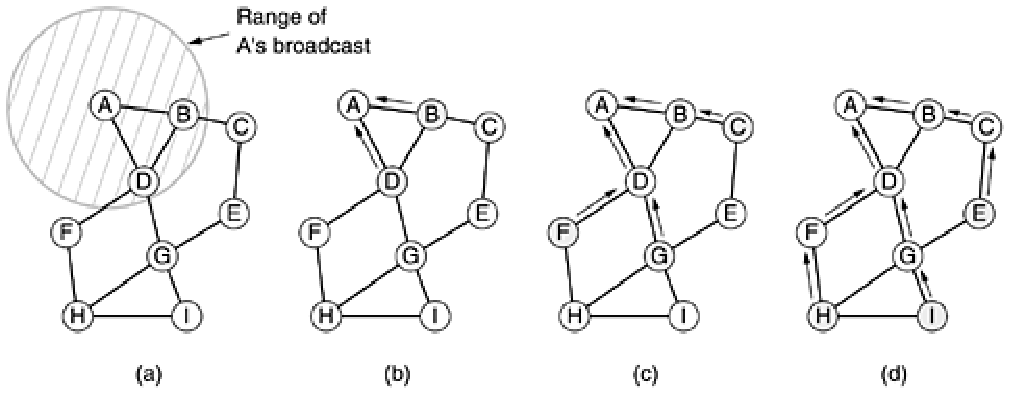
\includegraphics[scale=0.8]{images/pdf/AODV-tanenbaum-5-20.pdf}
		\caption{Vaiheet a--d Tanenbaumin kirjasta Computer Networks.}
		\label{fig:a-to-d}
	\end{center}
\end{figure}

Kuvassa (ks. \ref{fig:a-to-d}) näkyy reittipyynnön (\texttt{RREQ}) eteneminen verkossa vaiheittain, kun lähdesolmu A aloittaa reitin etsinnän. Vaiheessa (a) havainnollistetaan solmun A alkuperäisen yleislähetyksen kantamaa. Vaiheessa (b) pyyntö on saavuttanut solmut B ja D. Tämän jälkeen viesti etenee verkossa aaltona eteenpäin: vaiheessa (c) pyynnön ovat vastaanottaneet solmut C, F ja G, ja lopulta vaiheessa (d) solmut E, H ja I. Kuvassa varjostetut solmut kuvaavat kunkin vaiheen uusia vastaanottajia. Nuolet puolestaan osoittavat solmujen välille muodostuvia paluureittejä (engl. \textit{reverse routes}). Kun solmut välittävät \texttt{RREQ}-viestiä eteenpäin, ne tallentavat nämä paluureitit reititystauluihinsa, jotta mahdollinen \texttt{RREP}-vastausviesti osataan myöhemmin reitittää takaisin alkuperäiselle lähdesolmulle A. Jos viestin vastaanottava solmu on itse kohde (eli kuvaajassa I), tai sillä on reititystaulussaan tuore reitti kohteeseen, se lähettää takaisin \texttt{RREP}-vastausviestin (Route Reply) \cite{maurya-2012}. 

Reitin tuoreuden arvioimiseksi sekä reitityssilmukoiden (engl. \textit{routing loops}) estämiseksi AODV hyödyntää kohdesolmun sekvenssinumeroita (engl. \textit{destination sequence numbers}). Jokainen solmu ylläpitää omaa kasvavaa sekvenssinumeroaan. \cite{charles-1999}. Sekvenssinumero toimii eräänlaisena aikaleimana tuoreudesta. Lukua kasvatetaan aina RREQ:ta lähetettäessä sekä RREQ-viestiin vastatessa. Jälkimmäisessä tapauksessa kasvatuksen logiikka on max-operaatio, eli tee omasta sekvenssistä se luku, kumpi oli suurempi. \cite{maurya-2012}

Paluumatkan varrella olevat solmut tallentavat reittitiedot, mistä muodostuu reitti. Reittien tuoreutta vahditaan \texttt{HELLO}-viesteillä, jotka ovat tyyppiä lähialueen lähetys (engl. local broadcast) eli TTL (Time to Live) on 1 hyppy \cite{maurya-2012}. Hajonneista linkeistä viestitään RERR (Route Error) viestein \cite{maurya-2012}.

Toisin kuin monet edeltäjänsä, kuten Bellman-Ford, AODV ei tarvitse ajastetusti lähettäviä yleisviestejä, jotka sisältävät koko reititystaulun \cite{tanenbaum-2002}. Koska AODV välttää jatkuvia verkonlaajuisia reitityspäivityksiä ja ylimääräistä kontrolliliikennettä, se säästää solmujen akkuvirtaa ja on siksi soveltuva energiarajoitteisiin ympäristöihin. \cite{maurya-2012}

AODV skaalautuu rakenteelliseen yksinkertaisuuteensa nähden tehokkaasti. Mauryan ja kumppaneiden artikkelissa \cite{maurya-2012} käsitellään protokollan suorituskykyä, ja todetaan, että se soveltuu pääasiassa pienille ja keskisuurille verkoille, ja skaalauksen kattona on noin 1000 solmua. AODV luonnollisesti sopii verkoilla, joissa topologia vaihtuu tai on liikkuvuutta. Modernissa tutkimuksessa AODV:tä hyödynnetään esimerkiksi FANET-verkoissa (Flying Ad Hoc Networks), kuten drooniparvissa. Parvessa lentävät droonit voivat kommunikoida tätä protokollaa käyttäen. Tämä tieto on selvitetty Google Scholarissa tehtyjen hakujen avulla. Kumarin ja kumppaneiden artikkelissa \cite{kumar-2019} nostetaan erikseen esille ZigBee-pohjaisen sensoriverkot, joihin AODV sopi ainakin 2019 verrokkejaan paremmin.

Se, mihin AODV ei sovellu, ovat käänteisesti suuret eli yli 1000 solmun verkot tai etäisyyksien puolesta suuret verkot. Myös viivekriittisiin tehtäviin kannattaa valita proaktiviinen verkko mieluummin, mikäli mahdollista, koska reitin etsintä voi aiheuttaa viivettä. Lisäksi, jos tietoturvan suhteen on huolia, niin protokolla on altis hyökkäyksille \cite{maurya-2012} . Hyökkäysmielessä verkkoon liittyvä Solmu voi lähettää RREP-viestejä jokaista RREQ:ta vastaan ja täten saada pääsyn dataan \cite{security-2009}.

Zeng ja kumppanit \cite{wiley-2011} nostavat haittojen listalle myös sen, että se etsii lyhyimmän hyppyetäisyyden reittejä eikä välttämättä optimoi nopeutta, kuten myös sen, että "broadcast storm" on aito riski AODV:n kanssa.


% --------------------------------------------------  %
%                                                     %
%                  Esimerkki                          %
%                                                     %
% --------------------------------------------------- %

\chapter{Esimerkki}

Oletetaan, että verkko on juuri muodostettu ja sen reititystaulut ovat täysin tyhjiä. Solmu 1 haluaa lähettää viestin solmulle 6 (ks. Kuva \ref{fig:nodes}). Seuraava kuvaus perustuu Tanenbaumin kirjan hyvin vastaavaan esimerkkiin \cite{tanenbaum-2002}.

\begin{figure} [htbp]
	\begin{center}
		\leavevmode
		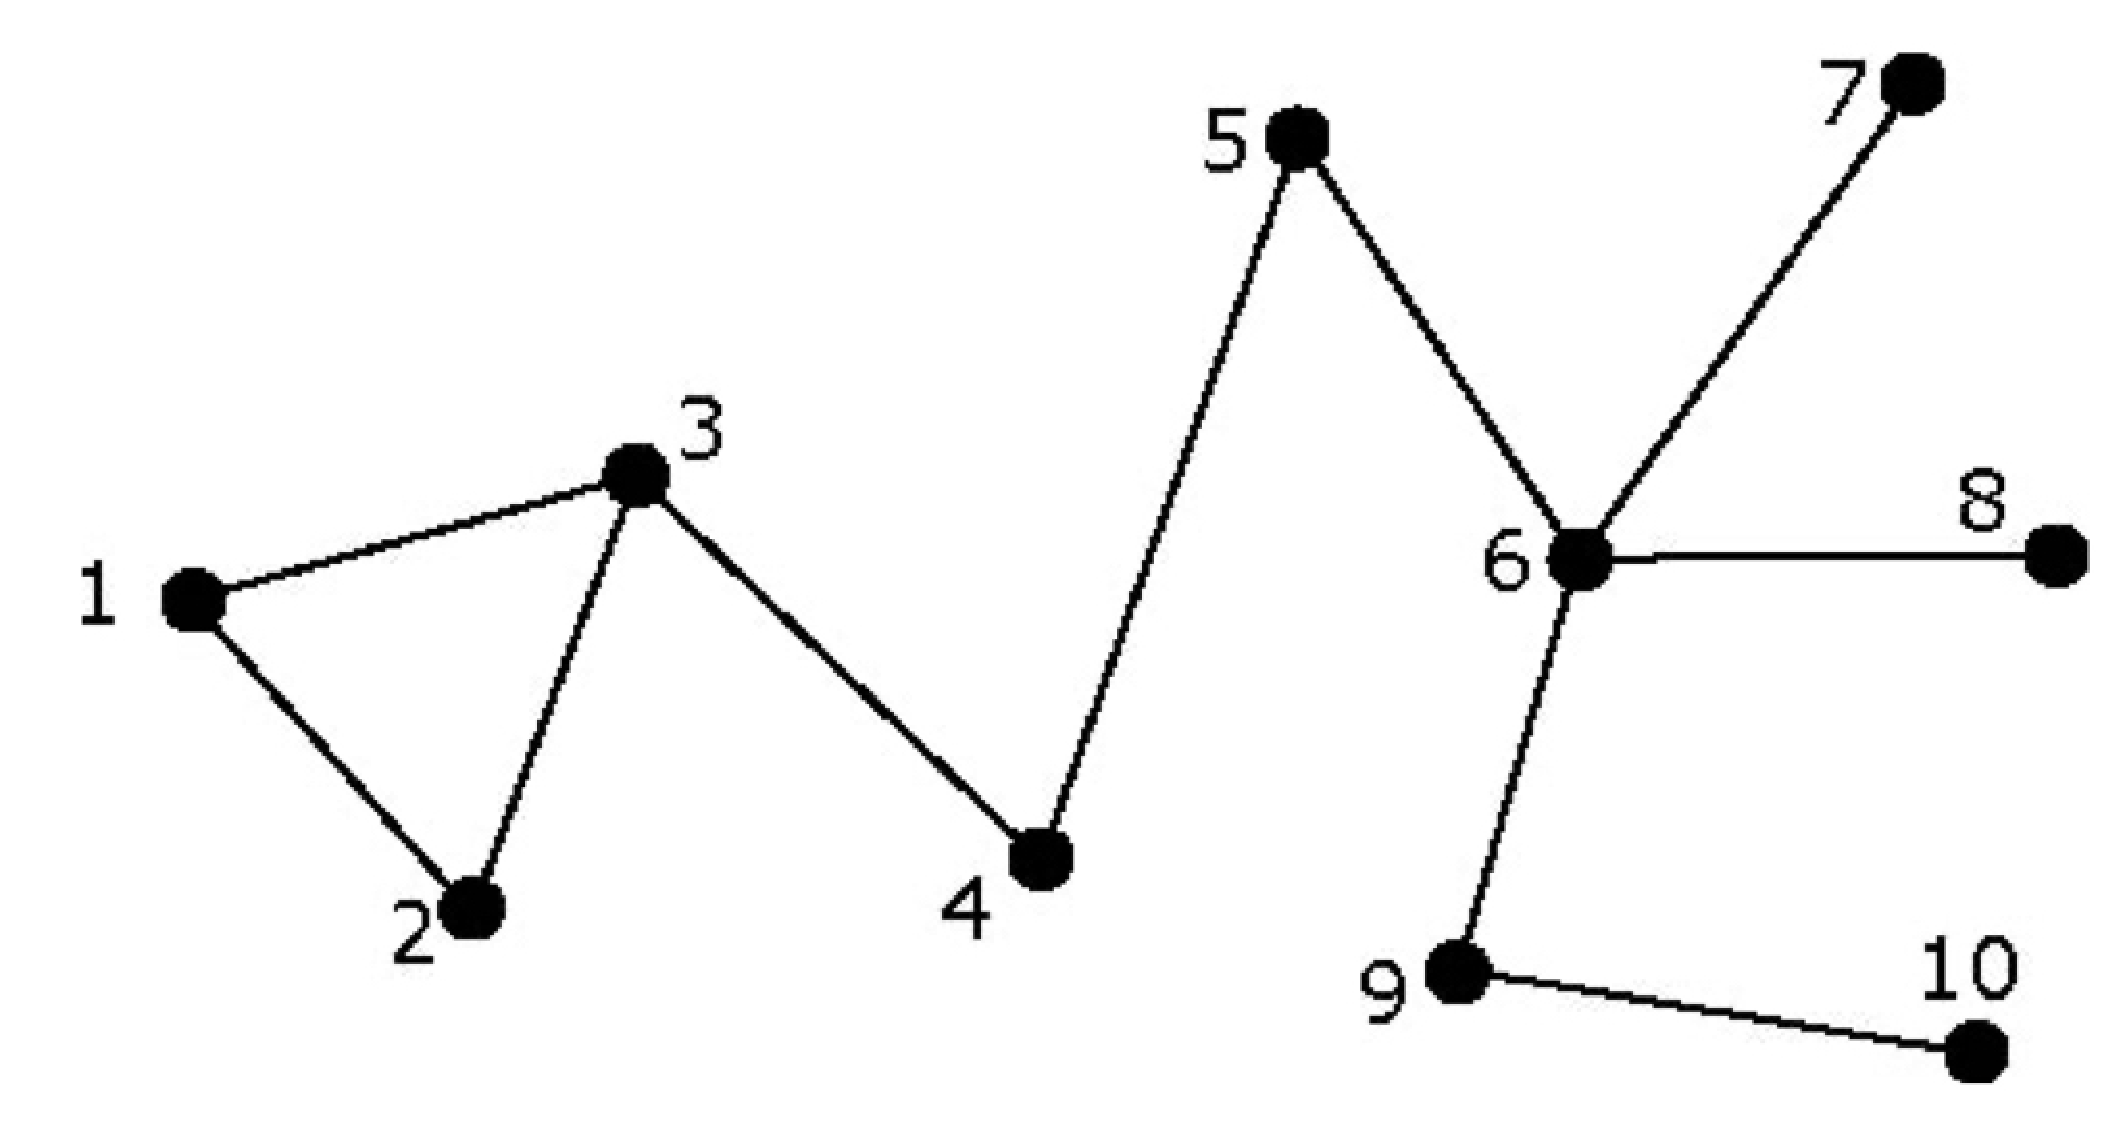
\includegraphics[scale=0.2]{images/pdf/AODV-assignment.pdf}
		\caption{Tehtävänannon verkko.}
		\label{fig:nodes}
	\end{center}
\end{figure}

Koska solmulla 1 ei ole reititystaulussaan tietoa solmusta 6, se aloittaa reitin etsinnän lähettämällä yleislähetyksenä reittipyynnön, kuten yllä on kirjoitettu. Tästä seuraa vaiheet, \textbf{Hyppy 1}, jossa Solmut 2 ja 3 vastaanottavat viestin. Kumpikaan ei tiedä reittiä, koska reititystaulut ovat yhä tyhjät. Kumpikin tallentaa historiatauluunsa viestin tunnisteen, jotta tunnistaa mahdollisesti verkossa kiertävät duplikaatit eli loopit. Kumpikin kasvattaa hyppyjen määrää ja välittää pyynnön eteenpäin. Lisäksi kumpikin tallentaa omaan käänteiseen reititystauluunsa (engl. reverse route table) rivin, jotta muistavat paluureitin. \textbf{Hyppy 2}, jossa Solmun 3 viesti saavuttaa Solmun neljä. Tässä tapahtuu samat vaiheet kuin yllä. Solmun 2 viesti päätyy Solmuille 1 ja 3, mutta kummatkin näistä tunnistavat sen duplikaattina. Tässä vaiheessa Solmu 4 tietää siis, että paluureitti Solmuun 1 on sellainen, jossa seuraava hyppy on Solmu 3. \textbf{Hyppy 3} on hyvin suoraviivainen äskeiseen verrattuna. Nyt \texttt{RREQ}-viestien edelleenlähestysketju (engl. rebroadcast) on edennyt Solmuun 5 asti. \textbf{Hyppy 4} Solmu 5 uudelleenlähettää viestin taas Solmu 4:lle, joka hylkää sen duplikaattina, mutta Solmu 6 reagoi siihen tähän asti uudella tavalla. Hän tunnistaa olevansa etsitty Solmu, ja aloittaa \texttt{RREP} eli vastausviestin lähettämisen. 

Kukin Solmu on tallentanut käänteiseen reititystauluunsa paluupostin kanavan, joten ne tietävät, kenelle se kuuluu lähettää. Tässä ei ole enää kyseessä broadcast vaan unicast: ellei Solmu ole kadonnut verkosta, lähettäjä tietää, että se on kuuloetäisyydellä. \texttt{RREP}-viesti palaa siis Solmuja pitkin reittiä 5, 4, 3 ja 1. Paluumatkalla kukin Solmu oppii reitin solmuun 6 lukemalla viestin hop counttia.

\begin{table}[htbp]
\centering
\begin{tabular}{cccc}
\toprule
\textbf{Solmu} & \textbf{Tunnettu kohde} & \textbf{Seuraava hyppy} & \textbf{Hyppyjen määrä} \\
\midrule
1 & Solmu 6 & Solmu 3 & 4 \\
\midrule
2 & Solmu 1 & Solmu 1 & 1 \\
\midrule
\multirow{2}{*}{3} & Solmu 1 & Solmu 1 & 1 \\
                   & Solmu 6 & Solmu 4 & 3 \\
\midrule
\multirow{2}{*}{4} & Solmu 1 & Solmu 3 & 2 \\
                   & Solmu 6 & Solmu 5 & 2 \\
\midrule
\multirow{2}{*}{5} & Solmu 1 & Solmu 4 & 3 \\
                   & Solmu 6 & Solmu 6 & 1 \\
\midrule
6 & Solmu 1 & Solmu 5 & 4 \\
\bottomrule
\end{tabular}
\caption{Solmujen reititystiedot operaation jälkeen.}
\label{tab:routing-table-1}
\end{table}

Seuraava skenaario esimerkissä on, että Solmu 1 haluaa lähettää viestin Solmulle 8, jota ei ole hänen reititystaulussaan (ks. Taulukko \ref{tab:routing-table-1}). Tulee siis lähettää uusi \texttt{RREQ}-viesti, jonka kohteena on Solmu 8. \textbf{Hyppy 1} -- \textbf{Hyppy 4} ovat identtiset edelliseen kertaan nähden. Ero syntyy vasta Solmun 6 kohdalla, eli kohdassa \textbf{Hyppy 5}. Tällä kertaa solmu ei tunnistaudu kohteeksi, vaan rebroadcastaa viestiä edelleen. Sen vastaanottavat Solmut 5, 7, 8 ja 9.  Solmu 5, aivan kuten aiemminkin, hylkää tämän duplikaattipaketin. Somuille 7, 8 ja 9 paketti on uutta tietoa. \textbf{Hyppy 6} -kohdalla Solmu 8 alkaa lähettää paluu- eli \texttt{RPEP}-viestiä ja samanaikaisesti Solmut 7 ja 9 jatkavat \texttt{RREQ}-viestin rebroadcastia, joka osin deduplikatoituu (9 -> 10 -> 9), osin aikakatkaistaan. Sen sijaan paluuviesti eli \texttt{RPEP} palaa Solmua 1 kohti käänteisreititystaulujen avulla eli reittiä 8, 6, 5, 4, 3, 1. Kaikki saavutettu tietous näkyy Taulukossa \ref{tab:routing-table-2}

\begin{table}[htbp]
\centering
\begin{tabular}{cccc}
\toprule
\textbf{Solmu} & \textbf{Tunnettu kohde} & \textbf{Seuraava hyppy} & \textbf{Hyppyjen määrä} \\
\midrule
\multirow{2}{*}{1} & Solmu 6 & Solmu 3 & 4 \\
                   & Solmu 8 & Solmu 3 & 5 \\
\midrule
2 & Solmu 1 & Solmu 1 & 1 \\
\midrule
\multirow{3}{*}{3} & Solmu 1 & Solmu 1 & 1 \\
                   & Solmu 6 & Solmu 4 & 3 \\
                   & Solmu 8 & Solmu 4 & 4 \\
\midrule
\multirow{3}{*}{4} & Solmu 1 & Solmu 3 & 2 \\
                   & Solmu 6 & Solmu 5 & 2 \\
                   & Solmu 8 & Solmu 5 & 3 \\
\midrule
\multirow{3}{*}{5} & Solmu 1 & Solmu 4 & 3 \\
                   & Solmu 6 & Solmu 6 & 1 \\
                   & Solmu 8 & Solmu 6 & 2 \\
\midrule
\multirow{2}{*}{6} & Solmu 1 & Solmu 5 & 4 \\
                   & Solmu 8 & Solmu 8 & 1 \\
\bottomrule
\end{tabular}
\caption{Solmujen reititystiedot toisen operaation jälkeen.}
\label{tab:routing-table-2}
\end{table}


\chapter{Yhteenveto}

AODV-protokollaan perehtymisen tuloksena on löydös, että kyseessä on reaktiivinen MANET-verkkoihin sunniteltu reititysprotokolla. Se muodostaa reittejä vain tarvittaessa. Sen ytimessä on reitinhaku, joka perustuu RREQ, RREP ja RERR viesteihin, sekä verkon reittien ylläpito, joka perustuu HELLO-viesteihin. Kukin noodi ylläpitää omaa reititystauluaan, joka syntyy reitinhaun kylkiäisenä, ja jossa kukin solmu esiintyy vain kerran. Tämä on energiatehokasta, ja siksi AODV toimii nimenomaan langattomiin sensoriverkkoihin, joissa laitteet ovat usein vähävirtaisia.

Kaikissa ratkaisuissa on omat rajoitteet tai tradeoffit, ja niin myös AODV:ssä. Protokollan skaalautuvuuden rajat ovat noin 1000 solmun kohdalla. Protokolla on myös altis broadcast storm -ilmiölle ja vihamielisille hyökkäyksille.

Esimerkissä näytettiin, kuinka duplikaattien hylkääminen tekee verkosta viestiluupeille immuunin, ja kuinka jo valmiiksi reititystaulussa olevat solmun rivit voivat nopeuttaa kauas ulottuvaa reitinhakua.


\chapter{Tekoälyn käyttö}

Käytin Github Copilot Pro:n Sonnet 4.6 mallia siihen, että muotoilin BibTeX-muotoiset lähteet OpenLMS:stä löytyvien merkkijonomuotoisten viitteiden avulla. Perkins & Belding -lähteen kävin etsimässä tosin valmiina BibTeXinä, kun se löytyi ResearchGatesta, mutta kahdesta muusta en löytäny valmista "Cite This"-nappia netistä. Tarkistin oikeellisuuden näistä silmämääräisesti. Vaihdoin muun muassa etu- ja sukunimien paikkaa, koska Kokkolan gradupohjan mallissa formaatti on tämä.

Lisäksi käytin samaa Sonnet-mallia taulukoiden muotoiluun: kirjoitin käsin CSV-tyylistä dataa, josta annoin kielimallin muovata oikeaa LaTeX-syntaksia.

Käytän kielimalleja lisäksi \textit{scaffolding}-tyylisessä työssä. Minulla on esimerkiksi Justfile-niminen skripti, joka kutsuu mogrifyä, joka kääntää kaikki alihakemiston PNG ja JPG kuvat oikeaan PDF-formaattiin. Tämä säästää turhaa käsityötä. Lopputulos on deterministinen skripti, joten sen oikeellisuus on helppo todistaa. Tähän työhön käytän ongelmasta riippuen joko Sonnetia tai GPT-5.4:ää Github Copilot Pro:n kautta. Kyseinen palvelu toimii nykyään enää vain opettajaksi tunnistautuneilla oikein; opiskelijat voivat käyttää vain karvalakkimalleja.

Tässä tehtävässä ei ole koodia, mutta jos olisi, niin koodin kirjoittamisessa käytän Github Copilot Pro:n lisäksi ajoitain myös OpenCodea, johon olen nykyisellään kytkenut CSC Aitta -inferenssipalvelun, jossa on useita avoimen lähdekoodin malleja, kuten 80 miljardin parametrin Qwen 3 Coder Next. Olen myös kokeillut pieniä, lokaalisti ajettavia malleja, mutta niiden suorituskyky ei yllä vielä sille tasolle, jossa kokisin ne hyödyksi. Suhtaudun agenttiseen koodariin pariohjelmoijana (engl. pair programming) tai minun alaisena. Luen ja tarkistan aivan kaiken koodin.

Lisälähteiden kartoittamiseen käytän O'Reilly Answer -mallia. Kyseessä on RAG, joka vastaa kysymyksiin O'Reillyn kirjastoon nojaten. Esitin sille kysymyksen "What is the basic idea in AOVD routing?". Malli toki vastasi jotakin myös, mutta itse vastaus ei minua suuremmin kiinnosta: minua kiinnostaa ne suorat linkit O'Reillyn kirjojen lukuihin, joissa kyseistä protokollaa käsitellään. Tämä palvelu on maksullinen ja vaatii O'Reillyn tilauksen (n. 500 e vuodessa).

Näiden lisäksi käytän Gemini 3.1 Pro:ta verkkoselaimen kautta. Käytän sitä haastamaan minun väitteitäni ja faktoja. En kopioi sen ehdotuksia suoraan, vaan otan ne tarkistettavina ehdotuksina. Käytännössä palaan alkuperäisen lähteen (esim. Perking & Belding tai Tanenbaum) äärelle ja tarkistan, olenko ymmärtänyt väärin.

Olen kokeillut opettajan työssä toistamiseen käyttää eri kielimalleja opetusmateriaalin tekemisen hyötynä. Toistaiseksi en ole vielä löytänyt mallia, jolle uskaltaisi jättää mitään paitsi kohtalaisen mekaanisia tehtäviä, kuten käännöstehtäviä, tekstin muotoilua esimerkiksi taulukoksi ja niin edelleen. Esimerkiksi tehtävänantojen runkoja tekoäly osaa kirjoittaa, kunhan vaatimukset on kirjattu listana, tai opettajan mallivastaus on tehty ja dokumentoitu, josta se voi poimia työvaiheet. Vastuu lopputuloksesta on luonnollisesti tekijällä eikä tekoälyllä, joten kaikki tulee tarkistaa ja hyväksyä.

\bibliography{KokkolaRaportti}

\end{document}
